\textbf{Model uczony na stałej krzywiźnie wierzechołków}

% \begin{figure}[ht]
% 	\centering
% 	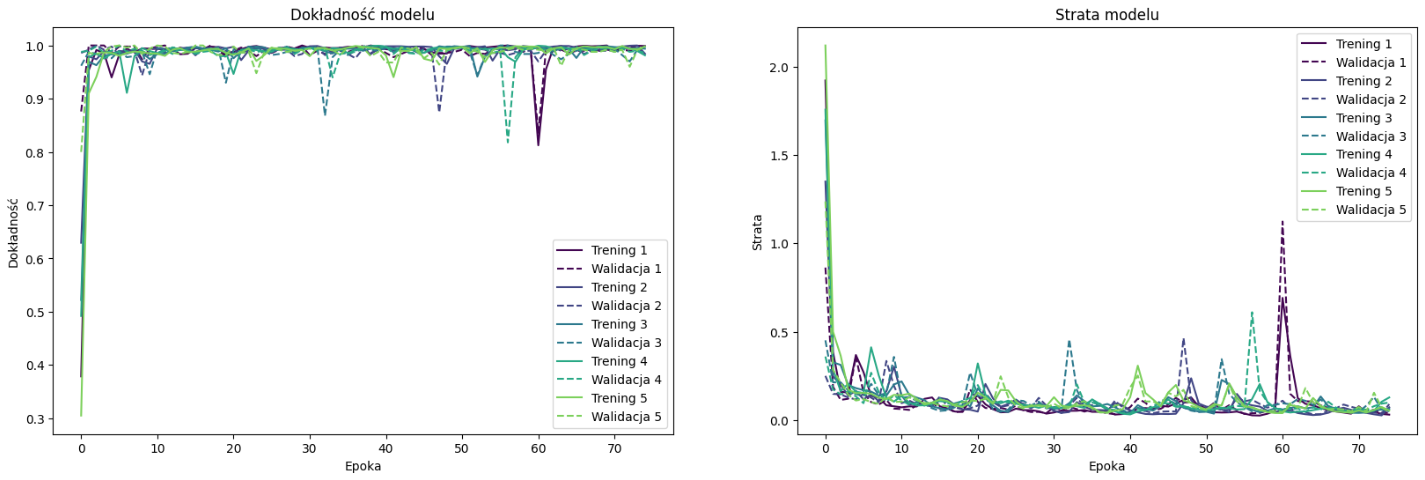
\includegraphics[height=5.5cm]{resources/tests/images/v2/multiple_edges_crossvalid_img.png}
% 	\caption{Wyniki testów dla modelu ze zmienną liczbą wierzchołków i walidacją krzyżową oraz stałą krzywizną wierzchołków}
% 	\label{Fig:tests-csvar-1}
% \end{figure}
% \FloatBarrier

% \begin{figure}[ht]
% 	\centering
% 	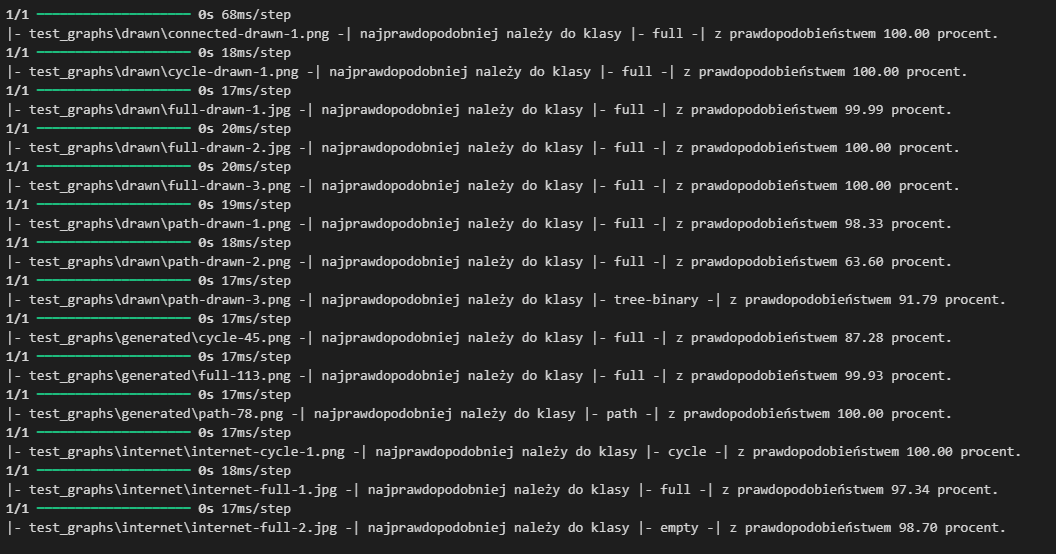
\includegraphics[height=5.5cm]{resources/tests/images/v2/multiple_edges_crossvalid_txt.png}
% 	\caption{Klasyfikacja obrazów zewnętrznych dla modelu ze zmienną liczbą wierzchołków i walidacją krzyżową oraz stałą krzywizną wierzchołków}
% 	\label{Fig:tests-csvar-2}
% \end{figure}
% \FloatBarrier

\textbf{Model uczony na losowej krzywiźnie wierzechołków}

Model uczony na grafach ze zmienną liczbą wierzchołków oraz zastosowaną walidacją krzyżową,
bardzo szybko osiąga poziom dokładności biski 100\%, bo już w kilku pierwszych epokach.
Po około 10 epoce, dokonuje się stabilizacja, oscylująca między 95\%, a 100\%.
W przypadku tego modelu, fluktuacje dokładności są znikome, co wskazuje na dobrą stabilność modelu.
Pojedyncze przypadku spadu dokładności, mogą być spowodowane bardziej skomplikowanymi
przypadkami w zbiorze danych walidacyjnych.

Strata tego modelu gwałtownie spada na początku procesu uczenia,
po czym stabilizuje się na zadowalająco niskim poziomie - poniżej 20\%.
Skoki wskaźnika są bardziej zauważalne na zbiorze walidacyjnym,
ale nie wydają się być regularne i nie wpływają na ogólny wynik.
Mogą być wynikiem, przeuczenia na pojedynczych epokach lub naturalną zmiennością walidacyjnego zbioru danych.

\begin{figure}[ht]
	\centering
	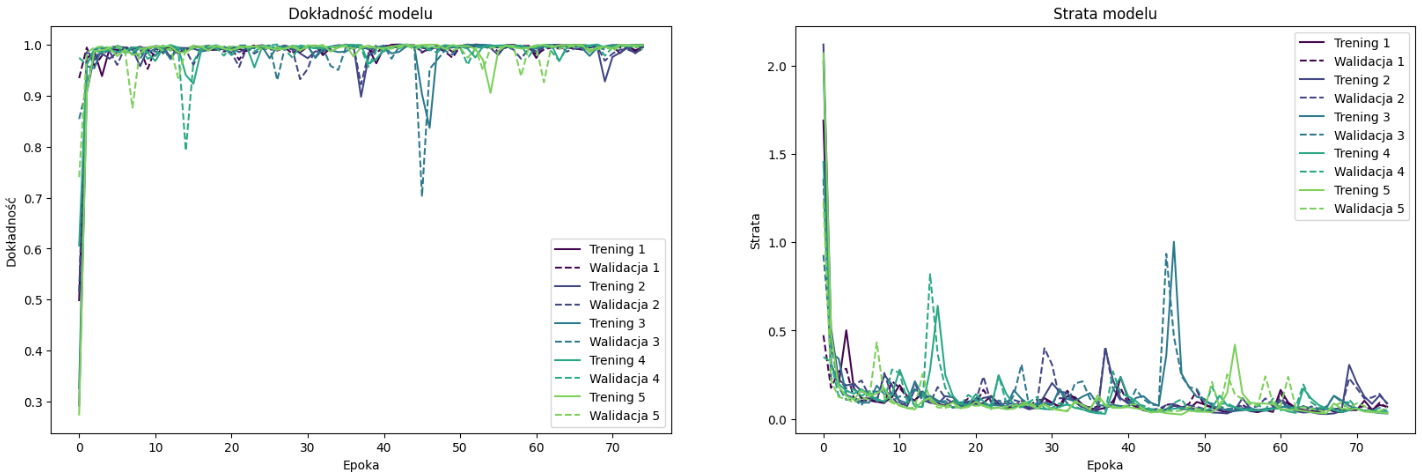
\includegraphics[height=5.5cm]{resources/tests/images/v3/multiple_edges_crossvalid_img.png}
	\caption{Wyniki testów dla modelu ze zmienną liczbą wierzchołków i walidacją krzyżową oraz losową krzywizną wierzchołków}
	\label{Fig:tests-csvar-1}
\end{figure}
\FloatBarrier

Model wydaje się dokładny na zbiorze treningowym i walidacyjnym,
co może skutkować polepszoną skutecznością w klasyfikacji grafów.
Minimalne różnice pomiędzy dokładnością treningową a walidacyjną wskazują na dobrą zdolność generalizacji.
Z otrzymanych wyników, wydawałoby się, że model nie uległ przeuczeniu,
choć jest to również możliwe, zważając na bardzo wysokie wyniki dokładności. 

\begin{figure}[ht]
	\centering
	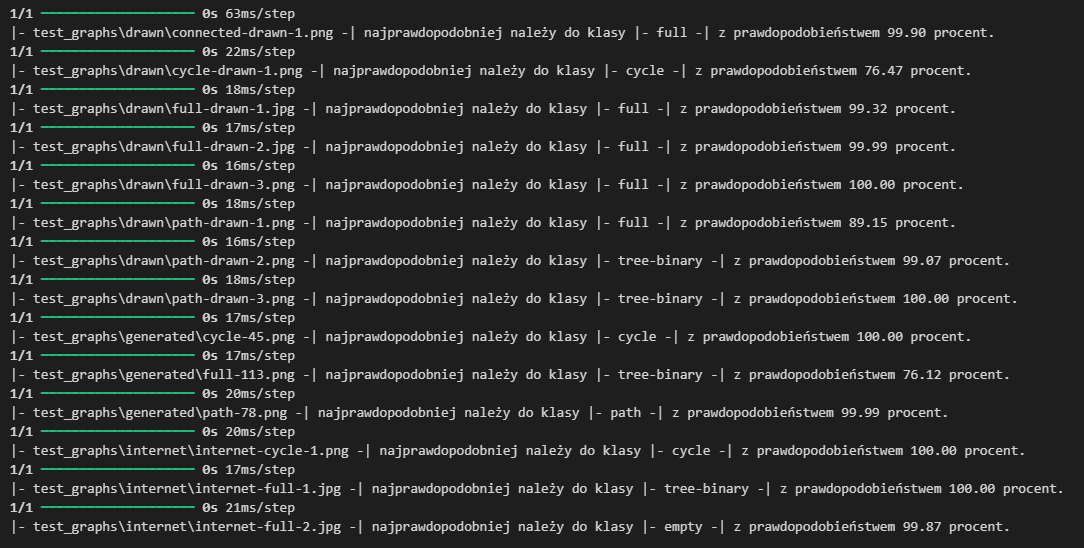
\includegraphics[height=5.5cm]{resources/tests/images/v3/multiple_edges_crossvalid_txt.png}
	\caption{Klasyfikacja obrazów zewnętrznych dla modelu ze zmienną liczbą wierzchołków i walidacją krzyżową oraz losową krzywizną wierzchołków}
	\label{Fig:tests-csvar-2}
\end{figure}
\FloatBarrier

Model poprawnie sklasyfikował połowę testowanych danych zewnętrznych.
Jest to zadowalający wynik, zważając na trudności innych modeli w poprawnym wskazywaniu klas sprawdzanych grafów.

\textbf{Zmodyfikowany model}

Opis modyfikacji % ------ TO DO ------ %

Dokładność % ------ TO DO ------ %

Strata % ------ TO DO ------ %

\begin{figure}[ht]
	\centering
	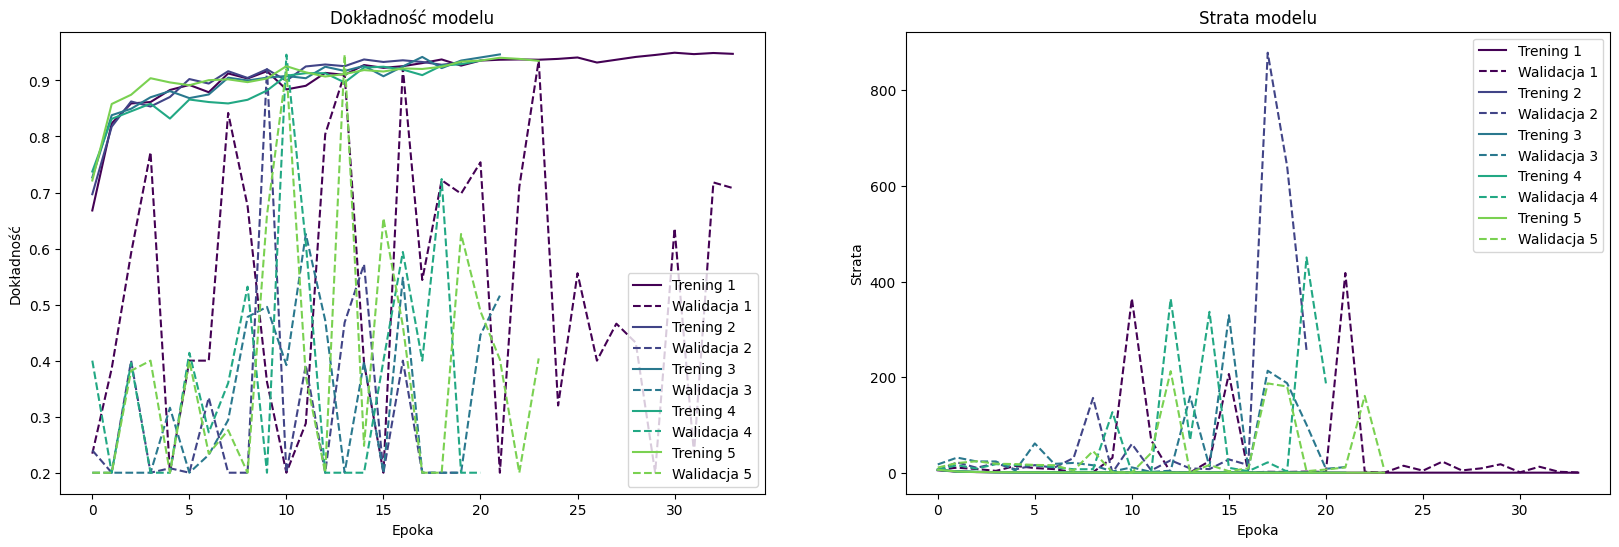
\includegraphics[height=7cm]{resources/tests/images/v4/multiple_edges_crossvalid_upgraded_img.png}
	\caption{Klasyfikacja obrazów zewnętrznych dla modelu z walidacją krzyżową i losową krzywizną wierzchołków}
	\label{Fig:tests-var-2}
\end{figure}
\FloatBarrier

Ogólne % ------ TO DO ------ %

\begin{figure}[ht]
	\centering
	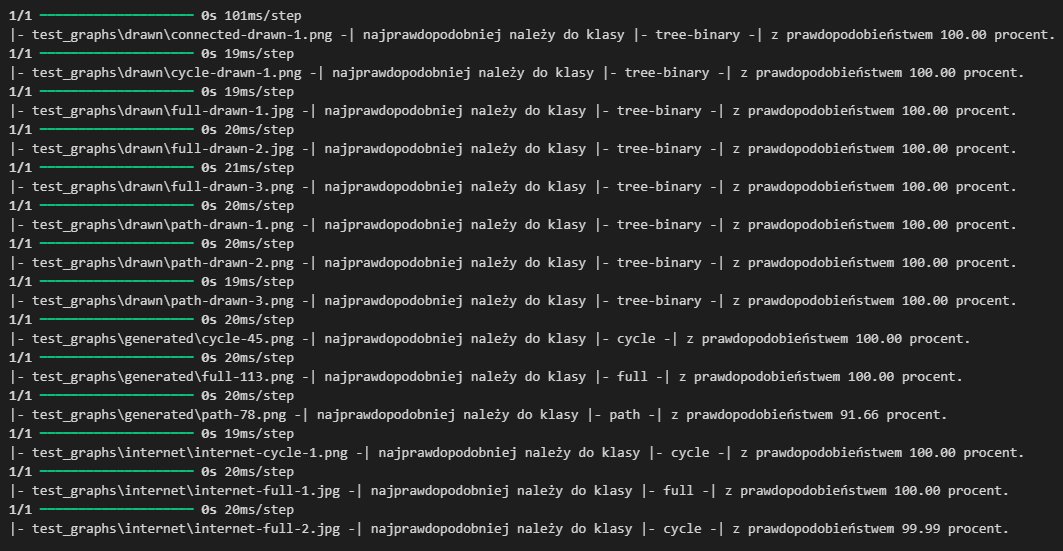
\includegraphics[height=7cm]{resources/tests/images/v4/multiple_edges_crossvalid_upgraded_txt.png}
	\caption{Klasyfikacja obrazów zewnętrznych dla modelu z walidacją krzyżową i losową krzywizną wierzchołków}
	\label{Fig:tests-var-2}
\end{figure}
\FloatBarrier

Opis klasyfikacji % ------ TO DO ------ %